\documentclass{article}

% Language setting
% Replace `english' with e.g. `spanish' to change the document language
\usepackage[english]{babel}
\usepackage{algpseudocode}
\usepackage{amsmath}
\DeclareMathOperator*{\argmax}{arg\,max}
\DeclareMathOperator*{\argmin}{arg\,min}

% Set page size and margins
% Replace `letterpaper' with `a4paper' for UK/EU standard size
\usepackage[letterpaper,top=2cm,bottom=2cm,left=3cm,right=3cm,marginparwidth=1.75cm]{geometry}

% Double Space
\usepackage{setspace}
\doublespacing

\usepackage[
backend=biber,
style=numeric,
sorting=nty
]{biblatex}
\addbibresource{sample.bib}

% Useful packages
\usepackage{amsmath}
\usepackage{graphicx}
\usepackage[colorlinks=true, allcolors=blue]{hyperref}

\title{Neurevolving Parameters for Vector Image Generation}
\author{Clint Wang}
\date{}
\begin{document}
\maketitle

\section{Introduction}

Current image generation learning methods such as diffusion and GANs are inadequate for high-precision image generation tasks. Raster images generated by such methods cannot be modified or adjusted if errors exist. Examples of this imprecision include artifacts in human hands, text, and diagrams. One possible solution to this is vector image generation for scientific diagrams, animating in-between frames, and text. 

This allows models to go over previously generated images and adjust control points, resolving artifacts. Existing gradient based learning methods have difficulty approximating a single spline, much-less multiple. This is because splines such as bezier curves require optimizing for multiple control points and it is easy for gradient-based methods to become stuck at a local optima. In this report, I propose a new learning method for generating vector images using neuroevolution. 

\begin{figure}[!ht]
\centering
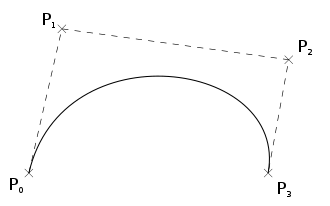
\includegraphics[width=0.7\textwidth]{bezier.png}
\caption{A bezier curve, one of the components commonly used in vector images, involves multiple control point vectors that can be modified. }
\end{figure}

\section{Methods}

Neuroevolution requires a constrained search space. For testing this learning method, the model consistes of a single feedforward layer, mapping pixels from an input $12\times12$ patch to a $12\times12$ probability map $P$, where $\rho_{(i, j)} \in [0, 1]$ represents the probability of a control point existing at that pixel. For approximating larger images, the model applies a sliding window $12\times12$ patch and evaluates the model on each patch, identifying possible curves that might exist in the image. 

\begin{figure}[!ht]
\centering
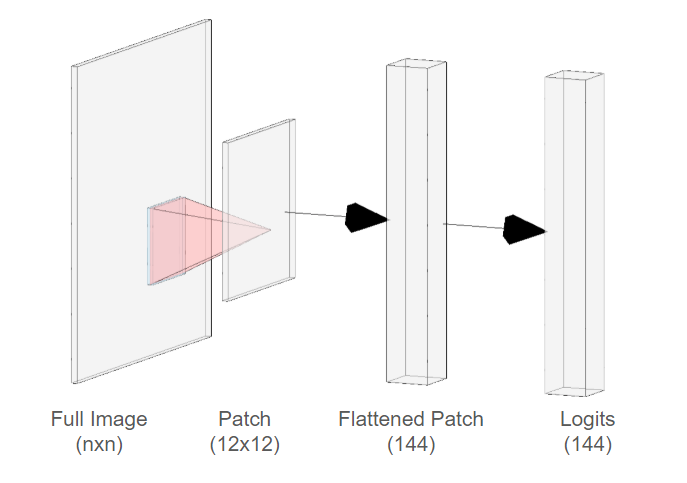
\includegraphics[width=0.7\textwidth]{model_arch.png}
\caption{Model architecture}
\end{figure}

\subsection{Optimization}

This model architecture leaves us with $20880$ parameters which is still pretty large for some evolutionary strategies. I found that CMA-ES, which stores the covariance matrix of parameters, yielding size $20880\times20880$ was extremely slow and memory inefficient for this task. Instead, I opted to use a simple tournament-based genetic algorithm. 

\begin{algorithmic}
\Procedure{Simple-GA}{$P, T$} \Comment{$P$: population, $T$: total tournaments}
    
    \For{$t \gets 1$ to $T$}
        \State Shuffle population indices
        \State $\text{pairs} \gets \text{partition\_into\_pairs}(P)$
        
        \For{$(i_1, i_2) \in \text{pairs}$}
            \If{$\text{loss}(i_1) = \text{loss}(i_2)$}
                \State $P[i_1] \gets P[i_2] + \text{noise}$
                \State \textbf{continue}
            \EndIf
            \If{$\text{loss}(i_1) > \text{loss}(i_2)$}
                \State Swap $i_1, i_2$
            \EndIf
            \State $P[i_1] \gets P[i_2] + \text{noise}$
        \EndFor
    \EndFor
\EndProcedure
\end{algorithmic}

\subsection{Fitness}
To evaluate the model, the loss function selects three control points based on the probability heatmap. A function permuates the control points and takes the lowest MSE to the actual control points.

\begin{equation}
\min_{\pi \in \Pi_3} \frac{1}{3} \sum_{i=1}^{3} \left(x_{i} - \hat{x}_{\pi(i)}\right)^{2}\label{eq:loss_calc}
\end{equation}
Where:
\begin{itemize}
\item $x_{i}$ represents the actual coordinates from the dataset
\item $\hat{x}{\pi(i)}$ represents the predicted coordinates
\item $\Pi_3$ is the set of all permutations of 3 coordinates
\item $\pi$ is a specific permutation mapping
\item $\min{\pi \in \Pi_3}$ finds the permutation that minimizes the Mean Squared Error
\end{itemize}

\begin{figure}[!ht]
\centering
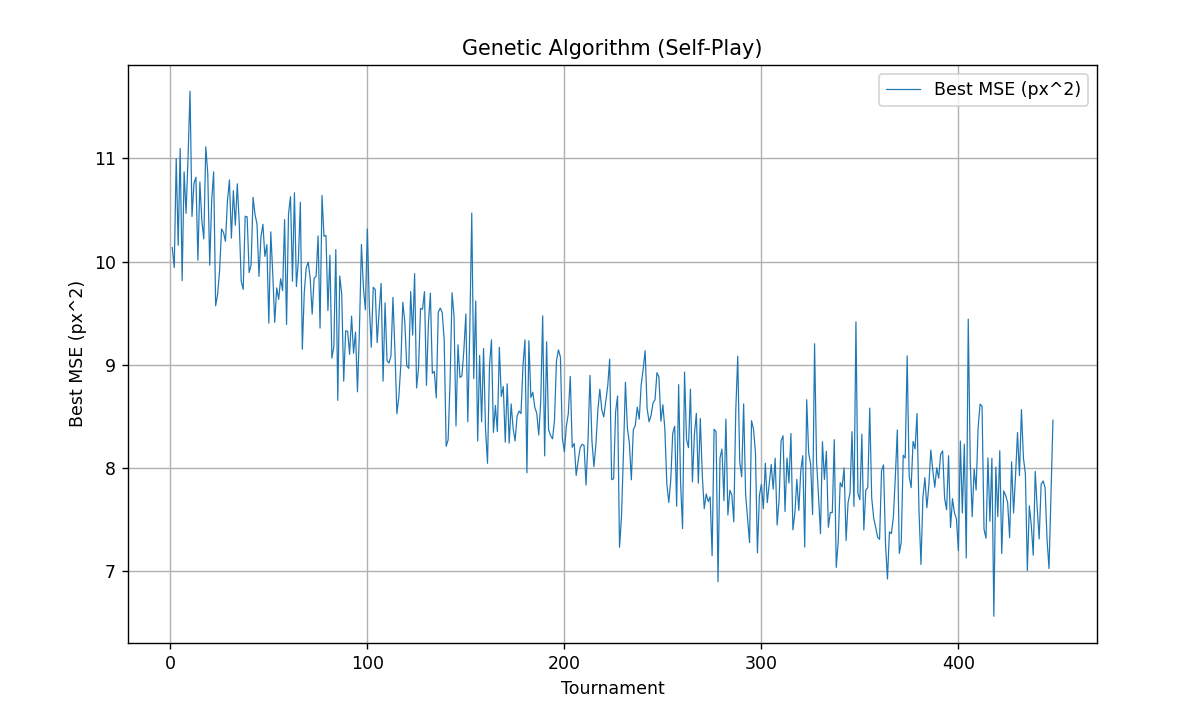
\includegraphics[width=0.7\textwidth]{ga-loss.png}
\caption{Loss curve in training Simple-GA over the course of 300 tournaments. }
\end{figure}

\section{Results}

The model trained by Simple-GA over 200 tournaments produced a MSE of 8.29 px whereas the model trained by gradient descent over 200 epochs produced a MSE of 9.46 px. This demonstrates an ability for simple-GA to generalize better to multiobjective learning problems in comparison to gradient descent.

\begin{figure}[!ht]
\centering
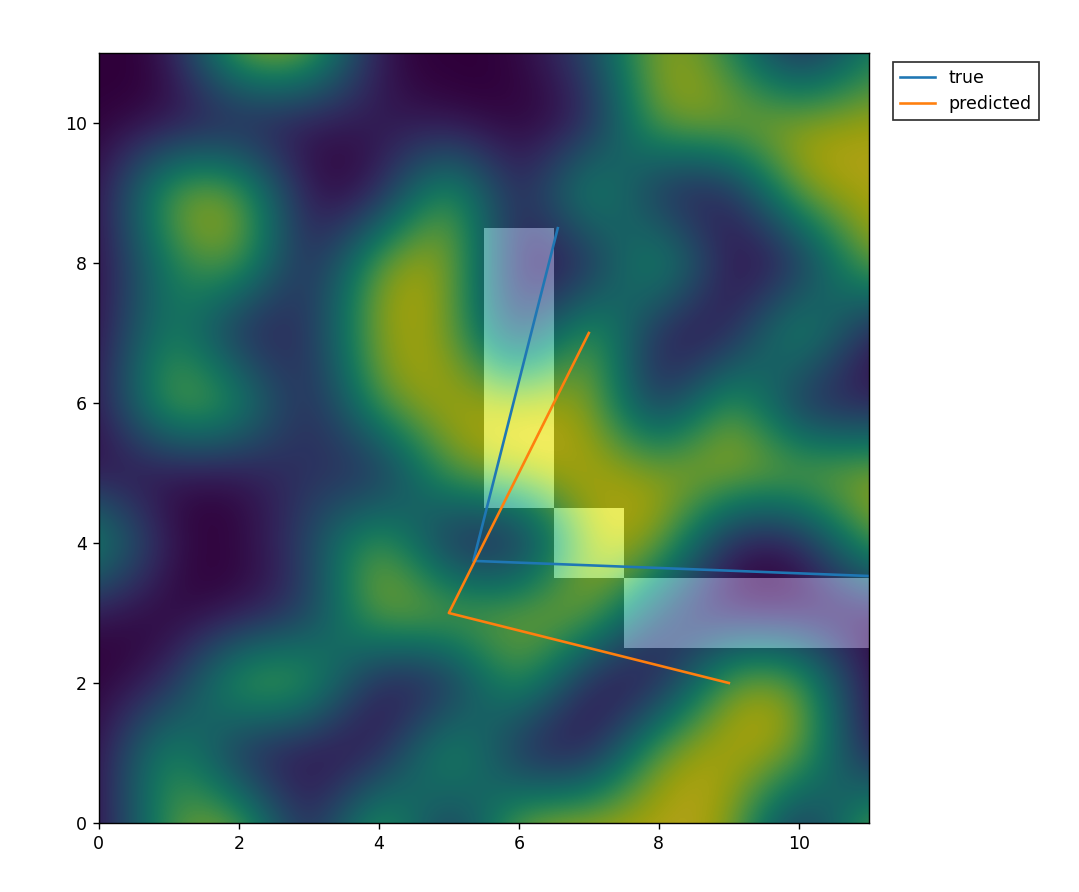
\includegraphics[width=0.7\textwidth]{sga-pred.png}
\caption{Example prediction made by the Simple-GA optimized model. The background heatmap displays the probability distribution created by the model. The control points are selected stochastically from the probability distribution and compared to the actual control points for the raster curve.}
\end{figure}

\section{Conclusion}

This simple experiment demonstrates the capability for neuroevolved learning methods to surpass gradient descent in the field of vector image generation. Next steps include optimizing the model and reducing parameter search space, running the model on larger images rather than just $12\times12$ patches. If this model and learning method demonstrates success with larger images, I would like to attempt to integrate LLMs to generate vector images through text rather than through image input.

\medskip

\printbibliography

\end{document}